\documentclass[main.tex]{subfiles}

\begin{document}

\lstset{
  basicstyle=\ttfamily\small,
  backgroundcolor=\color{gray!10},
  frame=single,
  breaklines=true,
  breakindent=0pt,
  xleftmargin=2em,
  framexleftmargin=1em,
  literate=
    {é}{{\'e}}1 {è}{{\`e}}1 {ê}{{\^e}}1 {à}{{\`a}}1 {ç}{{\c{c}}}1
    {’}{{'}}1 {‘}{{'}}1
    {“}{{\textquotedbl}}1 {”}{{\textquotedbl}}1
    {"}{{\textquotedbl}}1
    {_}{{\_}}1
}

\section{Partie Alexandre Picard}

\subsection{Introduction}

\quad Dans le cadre de ce projet, une application Windows Forms en C\# a été développée afin de gérer un système de lecture de tags via un port série. Le but principal est de fournir une interface utilisateur intuitive permettant la lecture, l'affectation de tag, l’identification et le suivi de données associées à des tags RFID, de façon structuré autour de plusieurs pages accessibles via un menu de navigation. Le développement s’est appuyé sur la migration d’un ancien projet en C++/CLI, avec pour objectif une meilleure maintenabilité, une gestion plus claire des ressources, et une modernisation de l’interface vers le C\#. Divers aspects techniques ont été abordés, notamment la gestion dynamique de l'affichage, l'intégration de ressources internes (images, textes), la lecture automatique depuis le bon port COM, ainsi que la structuration du code en couches logiques pour une meilleure réutilisabilité.

\subsection{Contextualisation}

Cette application dans le cadre du projet permet de centraliser les informations des visiteurs de façons sécuriser et qui permettra de gagner du temps lors de l'entrée de camion. Pour commencer la première interface disponible sera la connexion à la base de donnée. Suite à cela on on a l'interface Mainform qui permet le choix de Visiteurs déjà existant, de tags et de casiers pour la création d'une affectation. Si le visiteur n'est jamais venu alors il faudra créer ce visiteur à l'aide du menu qui permet d'accéder à une page de création de Visiteurs. De plus sur cette même page nous avons accès a la liste de casier disponible. L'utilisation décrite précédemment est la plus commune, mais en plus de cette description différente option sont disponibles dans le menu. Avec cette application on permet la simplification du trafic et une admission des chauffeurs plus rapide.

\begin{figure}[H]
	\centering
	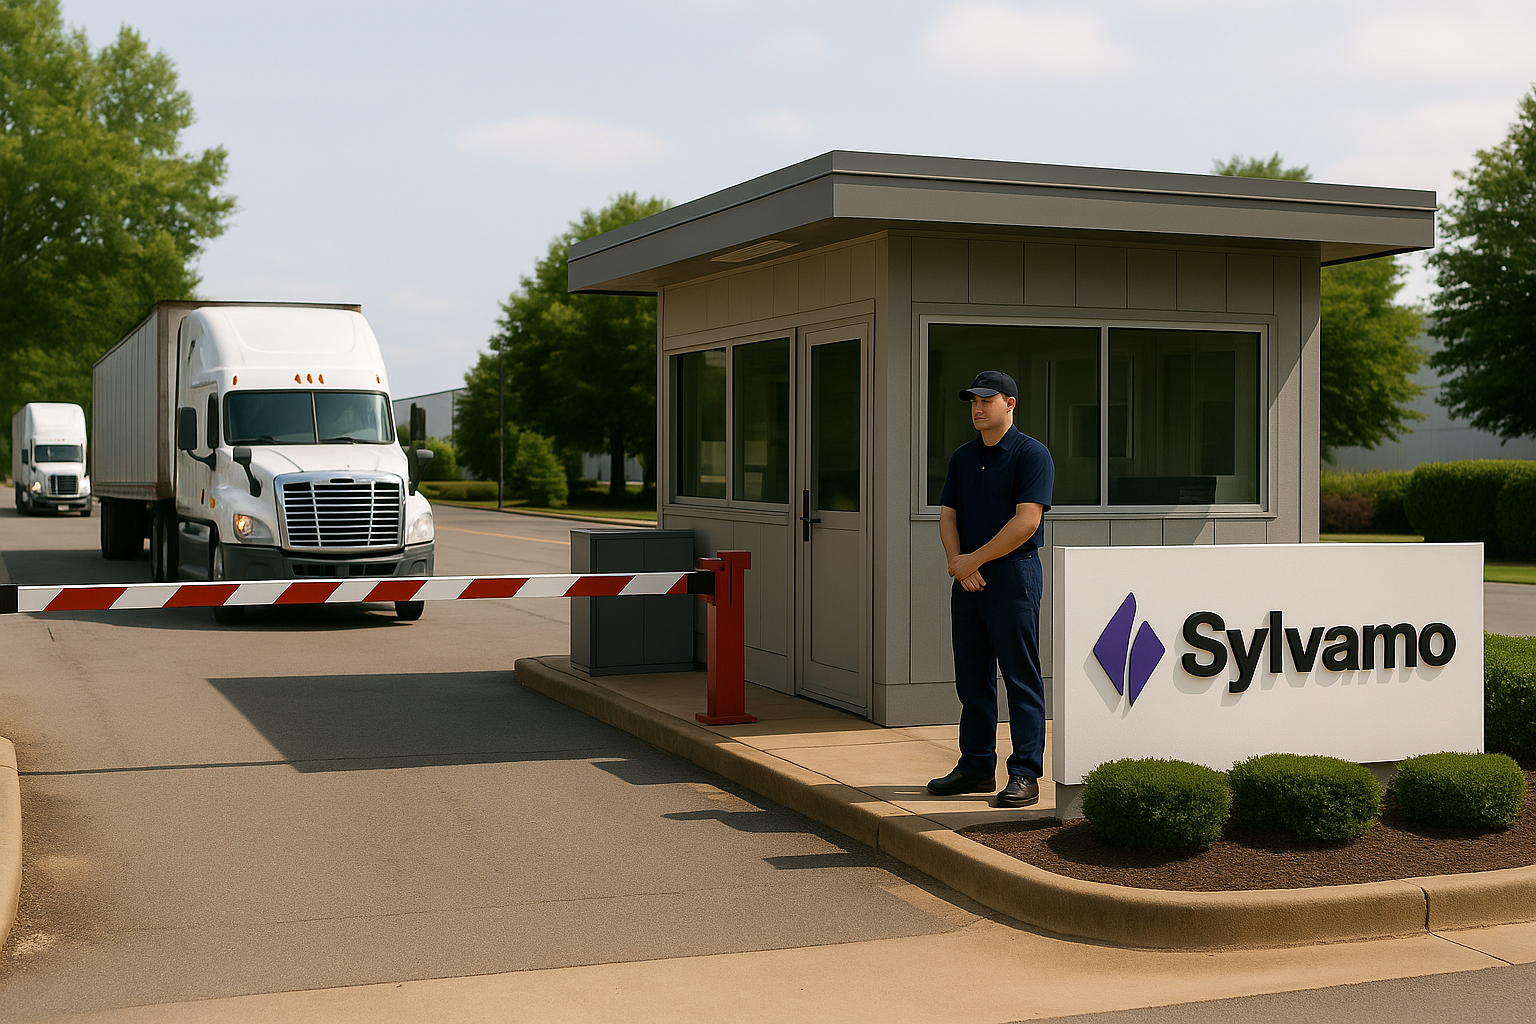
\includegraphics[width=0.7\textwidth]{../images/illusSylvamo}
	\caption{Image d'illustration}
	\label{fig:BDD_PP}
\end{figure}

\subsection{Base de donnée (MCD)}

Dans cette partie nous verrons la construction de la base de données et les tables qui la peuplent.  

\begin{figure}[H]
	\centering
	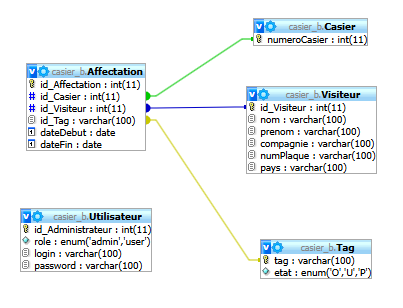
\includegraphics[width=0.7\textwidth]{../images/Base_de_donnee}
	\caption{Base de données}
	\label{fig:BDD_PP}
\end{figure}

Pour les tables nous avons la création de table Affectation qui regroupe 3 autres classes : 

\begin{itemize}
\item Tag 
\item Visiteur  
\item Casier 
\end{itemize}

Affectation aura donc des clés secondaires pour chacune de ces tables il sera composé par un id propre qui sera une clé primaire puis celui de la clé primaire de classe Tag qui sera secondaire ainsi de même pour la classe Visiteur et la classe Casier. 

A côté de cela on a la base de données Utilisateur qui permettra de donner à un utilisateur un rôle d’admin ou bien d’utilisateur classique. Du côté de l’application de cette différence donnera plus de droit au admin concernant les tables. 

\textbf{Table Tag :}

La table Tag contient les identifiants des badges ou étiquettes (souvent RFID) utilisés pour accéder aux casiers. Chaque tag est identifié de manière unique par une chaîne de caractères (tag). Un champ etat précise la situation du tag à un moment donné : 

\begin{itemize}
\item 'O' pour occuper : le tag est actuellement utilisé pour un casier en service
\item 'U' pour utilisable : le tag est disponible pour une nouvelle affectation
\item 'P' pour perdu : le tag est déclaré perdu et ne doit plus être utilisé\\
\end{itemize}
 
\textbf{Table Visiteur :}

La table Visiteur stocke les informations relatives aux personnes qui utilisent les casiers. Chaque visiteur possède un identifiant unique (id\_Visiteur) généré automatiquement. Les autres informations incluent : 

\begin{itemize}
\item Le nom et le prénom du visiteur
\item Le nom de la compagnie à laquelle il est affilié  
\item Le numéro de plaque d’immatriculation de son véhicule
\item Le pays d’origine du visiteur\\
\end{itemize}

\textbf{Table Casier :}

Cette table contient la liste des casiers disponibles. Chaque casier est identifié par un numéro (numeroCasier) qui sert également de clé primaire. Aucun autre attribut n’est stocké ici pour le moment. 

\textbf{Table Affectation :}

La table Affectation représente l'historique ou l'enregistrement des prêts de casiers aux visiteurs. Elle fait le lien entre un casier, un visiteur, et un tag, en précisant également la période d'utilisation. Chaque affectation possède un identifiant unique (id\_Affectation) auto-incrémenté. 

Les colonnes incluent : 
\begin{itemize}
\item id\_Casier : fait référence au casier attribué (clé étrangère liée à Casier) 
\item id\_Visiteur : identifie le visiteur concerné (clé étrangère liée à Visiteur)  
\item dateDebut et dateFin : représentent la durée pendant laquelle le casier est affecté \\
\end{itemize}

\textbf{Table Utilisateur :}

La table Utilisateur contient les informations sur les personnes pouvant accéder à l’interface de gestion de la base de données. Chaque utilisateur a un identifiant unique (id\_Administrateur) auto-incrémenté. 

Les autres champs sont : 
\begin{itemize}
\item role : précise le rôle de l’utilisateur, qui peut être admin (administrateur) ou user (utilisateur simple)
\item login : identifiant de connexion 
\item password : mot de passe (idéalement, ce champ devrait être chiffré ou haché pour des raisons de sécurité, ce que la structure actuelle ne gère pas encore) \\
\end{itemize}
 

Pour les bases de données on a chiffré les informations personnelles comme celles des utilisateurs de l’application ainsi que les visiteurs. Nous avons cependant laissé les Tags, les Casiers ainsi que les affectations non chiffrer. 

Cette base de données est implantée sur une base de données qui sera au préalable crée sur une raspberry pi avec mariaDB. 

\textbf{Insertion :}

Pour les tests de l'application nous aurons besoin d'information qui sois déjà existante, pour ce faire on insère :

\begin{itemize}
\item un administrateur
\item des visiteurs 
\item les 4 casiers existant
\item les tags possédés 
\item des affectations qui relis les exemples entres eux
\end{itemize}


\subsection{Application C++/CLI}

Cette application a commencer par ce language car il a été étudié lors de nos cours dans le cadre du BTS. Pour commencer nous verrons ce qu'est le C++/CLI.

\subsubsection{Qu'est ce que le C++/CLI}

Le C++/CLI est une extension du langage C++ développée par Microsoft pour fonctionner avec la plateforme .NET. Il combine le C++ traditionnel (dit natif) avec des fonctionnalités propres au monde managé de .NET. Contrairement au C++ standard, qui est compilé directement en code machine et utilise une gestion manuelle de la mémoire, le C++/CLI s'exécute dans l’environnement .NET via le Common Language Runtime (CLR), et utilise des types managés (comme String\^{}).

Cela permet au C++/CLI de servir de passerelle entre des bibliothèques natives en C++ et des applications écrites dans des langages .NET comme C\#. On peut ainsi, dans une même application, manipuler à la fois des objets classiques du C++ (comme std::string) et des objets managés du .NET Framework (comme System::String\^{}).

Le C++/CLI permet d'intégrer du code C++ existant dans un environnement .NET tout en bénéficiant de l'interopérabilité et de la gestion mémoire automatique du CLR. C'est un langage puissant pour faire la liaison le code et l'applicatif.

\subsubsection{Première application}

Cette application, développée en C++/CLI avec Windows Forms, avais pour objectif de gérer l’accueil et le suivi de visiteurs dans un environnement sécurisé. Elle s’articule autour de plusieurs fonctionnalités clés, intégrées progressivement au cours du développement.

\textbf{Interface graphique}

L’interface utilisateur repose sur Windows Forms, ce qui permet la création de formulaires interactifs, avec une navigation fluide entre différentes pages (accueil, ajout de visiteur, etc.). L’application utilise des panneaux (Panel) dynamiques ou un menu de type hamburger pour organiser et afficher les différentes sections sans devoir ouvrir de nouvelles fenêtres. Des boîtes de dialogue (MessageBox) sont également utilisées pour interagir avec l’utilisateur, notamment pour la saisie d’informations telles que le login et le mot de passe, ou pour confirmer certaines actions (ex. : fermeture de l’application).

\textbf{Connexion à la base de données}

L’application communique avec une base de données MariaDB ou MySQL à l’aide d’ADO.NET, grâce au MariaDB Connector/NET ou au MySQL Connector/NET. Ce choix permet une compatibilité directe avec le modèle ADO.NET intégré à .NET, facilitant l’exécution de requêtes SQL.

Les opérations de lecture et d’écriture (ex. : ajout d’un visiteur) sont réalisées via des objets comme MySqlConnection et MySqlCommand. Pour sécuriser les requêtes et éviter les injections SQL, l’utilisation de requêtes préparées est recommandée.

\textbf{Lecture via port série}

L’application intègre un module de lecture de tags RFID ou d’identifiants via un port série (COM). Ce module vise à détecter automatiquement le port série utilisé et à lire les données reçues. La gestion de ce lecteur est encapsulée dans une classe dédiée, qui pourra être intégrée de manière fluide à l’interface et aux autres modules de l’application.

\textbf{Sécurité et cryptage}

Dans un souci de sécurité, une classe de cryptage/décryptage est en cours d’élaboration pour chiffrer certaines données sensibles (comme les mots de passe). L’approche choisie privilégie une méthode simple et autonome, sans nécessiter de bibliothèques externes. L’objectif est d’implémenter une méthode de chiffrement symétrique légère, suffisante pour un stockage sécurisé local sans dépendances tierces.

\textbf{Gestion des erreurs}

Des erreurs de type NullReferenceException ont été rencontrées, généralement causées par l’utilisation d’objets non initialisés (m\_stmt, m\_conn).

Voici ce que cela donne pour l'application :

\begin{figure}[H]
	\centering
	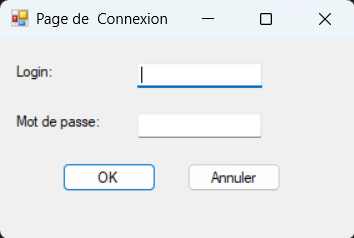
\includegraphics[width=0.6\textwidth]{../images/ConnexionCLI}
	\caption{Page de connexion à l'application}
	\label{fig:C_CLI}
\end{figure}

\begin{figure}[H]
	\centering
	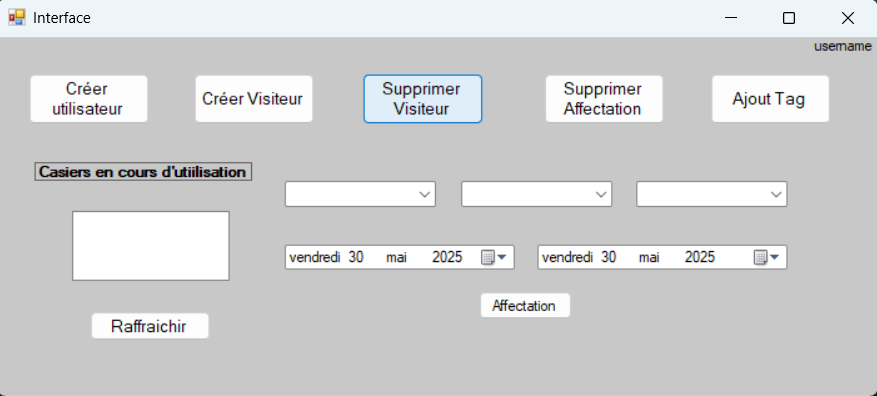
\includegraphics[width=0.9\textwidth]{../images/AppCLI}
	\caption{Interface de l'application Administrateur}
	\label{fig:AA_CLI}
\end{figure}

\begin{figure}[H]
	\centering
	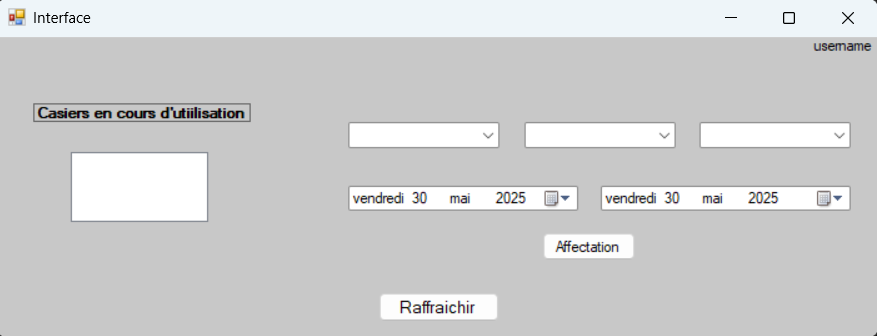
\includegraphics[width=0.9\textwidth]{../images/AppUserCLI}
	\caption{Interface de l'application Utilisateur}
	\label{fig:AU_CLI}
\end{figure}

\begin{figure}[H]
	\centering
	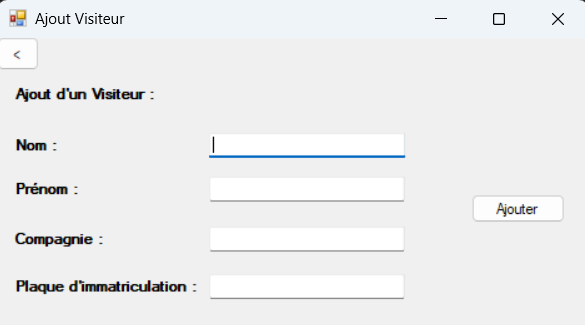
\includegraphics[width=0.8\textwidth]{../images/AjoutVisiteurCLI}
	\caption{Page d'ajout de Visiteur}
	\label{fig:AV_CLI}
\end{figure}

\begin{figure}[H]
	\centering
	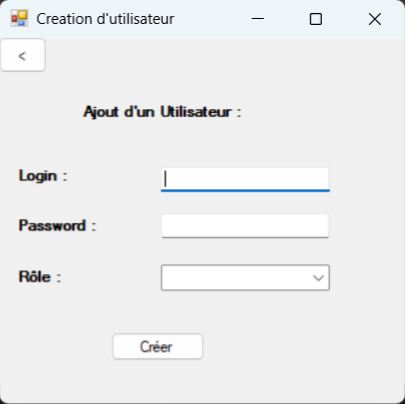
\includegraphics[width=0.6\textwidth]{../images/AjoutUserCLI}
	\caption{Page d'ajout d'utilisateur}
	\label{fig:AUA_CLI}
\end{figure}

\subsubsection{Transition vers le C\#}

Le passage du C++/CLI vers le C\# s’explique principalement par la volonté de simplifier le développement et d’améliorer la maintenabilité du code. Bien que le C++/CLI permette de tirer parti de bibliothèques C++ natives tout en accédant à l’environnement .NET, il reste plus complexe à lire et à écrire, notamment à cause de sa syntaxe hybride mêlant gestion manuelle et managée de la mémoire.

Migrer vers C\# permet donc d’obtenir un code plus lisible, plus robuste, et plus facile à maintenir, tout en s’alignant sur les standards actuels du développement logiciel.

De plus la taille de l'application avec est bien plus grosse pour une petite application  comme celle ci. 

\begin{figure}[H]
	\centering
	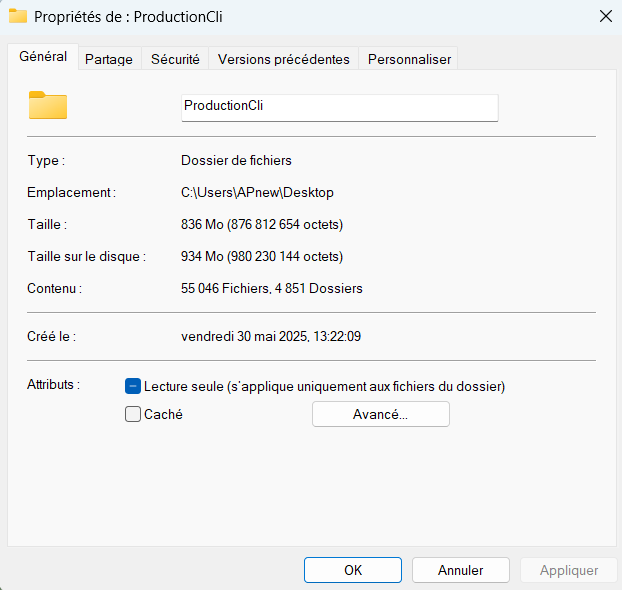
\includegraphics[width=0.7\textwidth]{../images/Taille_CLI}
	\caption{Taille du dossier C++/CLI}
	\label{fig:TD_CLI}
\end{figure}

Contrairement au nouveau projet qui a un coût en place bien moins élever. 

\subsection{Application C\#}

Après une première version de l’application réalisée en C++/CLI, le choix a été fait de migrer le projet vers le langage C\#. Cette transition s’inscrit dans une logique de modernisation et de simplification du développement. C\# offre un environnement de programmation plus intuitif, mieux adapté aux applications modernes et à la gestion d’interfaces utilisateur. Ce langage, totalement intégré à l’environnement .NET, permet également une meilleure organisation du code, une maintenance facilitée, ainsi qu’une exploitation plus efficace des bibliothèques et outils récents.

Voici le plan de l'application qui permet de voir les différentes possibilités : 

\begin{figure}[H]
	\centering
	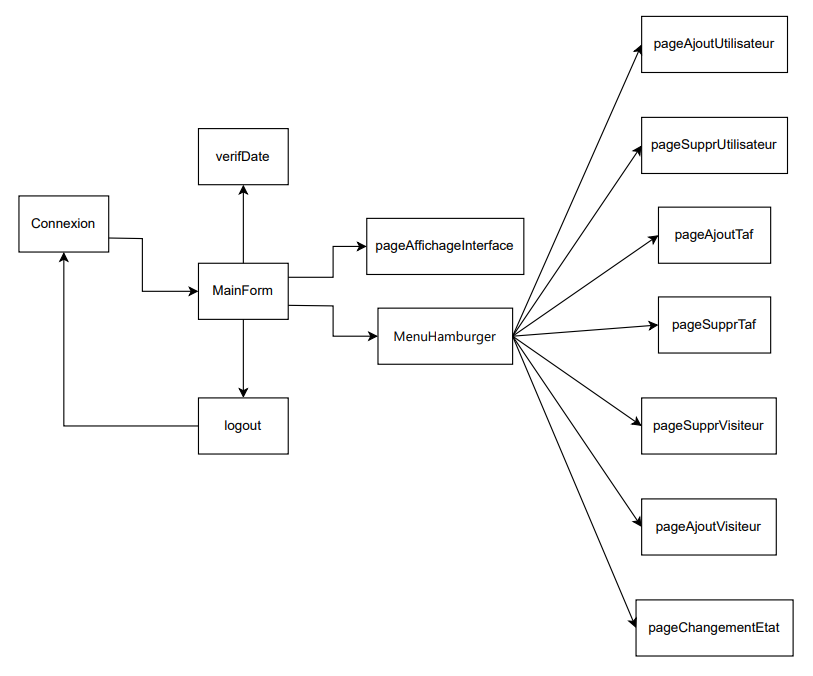
\includegraphics[width=0.9\textwidth]{../images/AppShema}
	\caption{Shéma de l'application}
	\label{fig:APPS}
\end{figure}

\subsubsection{Qu'est ce que le C\#}

C\# est un langage de programmation orientée objet, fortement typé, dérivé de C et de C++, ressemblant au langage Java. Il est utilisé pour développer des applications web, ainsi que des applications de bureau, des services web, des commandes, des widgets ou des bibliothèques de classes. En C\#, une application est un lot de classes où une des classes comporte une méthode Main, comme cela se fait en Java.

C\# est destiné à développer sur la plateforme .NET, une pile technologique créée par Microsoft pour succéder à COM.

Les exécutables en C\# sont subdivisés en assemblies, en namespaces, en classes et en membres de classe. Un assembly est la forme compilée, qui peut être un programme (un exécutable) ou une bibliothèque de classes (une dll). Un assembly contient le code exécutable en MSIL, ainsi que les symboles. Le code MSIL est traduit en langage machine au moment de l'exécution par la fonction just-in-time de la plateforme .NET.

C\# est destiné à développer sur la plateforme .NET. Le cœur de cette pile technologique est le framework .NET, composé de :

\begin{itemize}
\item Les environnements ASP.NET et Winforms (qui servent à exécuter respectivement des applications web et de bureau) conçus pour la plateforme .NET;
\item Une bibliothèque de classes qui permet de manipuler des fichiers, manipuler des tableaux ou des structures en arbres, accéder à Internet, créer des interfaces graphiques, accéder à des bases de données, accéder au registre Windows et beaucoup d'autres choses. La plupart des fonctionnalités sont offertes par des classes de l'espace de noms System ;
\item Le Common Language Runtime (CLR) est le runtime utilisé par les langages de la plateforme .NET (C\#, Visual Basic .NET, J\#, etc.), les services fournis par la CLR sont le lancement et l'exécution de programmes, le ramasse-miettes et la gestion d'exceptions. Un programme pour la plateforme .NET est tout d'abord compilé en une forme intermédiaire, le MSIL, puis ce code MSIL est transformé en code machine qui sera exécuté par la CLR. Ce code machine est appelé managed code parce que son exécution est sous le contrôle de la CLR.
\end{itemize}

Un autre produit de la plateforme .NET est l'environnement de développement Visual Studio .NET, outil généralement utilisé pour programmer en C\#.

\subsubsection{Classe pour la base de données}

Ce code implémente une classe DatabaseConnection.cs  qui permet de gérer la connexion à une base de données MySQL et d'interagir avec celle-ci. Il utilise C\# et la bibliothèque MySqlConnector pour établir des connexions et exécuter des requêtes SQL.  

MySqlConnector est un client MySQL performant et optimisé pour les applications .NET. Il présente plusieurs avantages notables, notamment une bonne gestion des connexions, une compatibilité parfaite avec C\#, une utilisation simple et intuitive, et une grande rapidité dans l'exécution des requêtes. De plus, étant open-source et gratuit, il permet de réduire les coûts. MySqlConnector est donc idéal pour des projets nécessitant une interaction rapide et fiable avec une base de données MySQL, ce qui justifie son choix dans ce projet.  

Une fonction typique de connexion à une base de données en C\# avec MySqlConnector commence par la définition d’une chaîne de connexion. Cette chaîne contient les informations nécessaires pour atteindre la base (serveur, utilisateur, mot de passe, base ciblée). Ensuite, un objet de connexion est instancié à partir de cette chaîne. La connexion est ouverte à l’intérieur d’un bloc try, ce qui permet d’intercepter les éventuelles erreurs via un bloc catch. En cas de succès, la connexion est retournée pour être utilisée ailleurs dans le programme. 

La fermeture de la connexion est tout aussi importante. Elle se fait en appelant la méthode .Close() ou, de manière plus sûre, en utilisant un bloc using, qui garantit la libération automatique des ressources même en cas d’erreur. Cela évite les fuites mémoire ou les connexions persistantes non libérées, qui pourraient nuire aux performances ou à la stabilité de l’application. 

La classe se concentre principalement sur la gestion de données liées à des utilisateurs, des visiteurs et des casiers dans un système. Elle inclut des fonctionnalités telles que l'ajout et la suppression d'utilisateurs, la vérification des rôles (administrateurs) et l'affectation de casiers à des visiteurs. 

Les informations sensibles, comme les mots de passe, sont sécurisées via un chiffrement personnalisé basé sur la méthode XOR, garantissant ainsi la confidentialité des données stockées.  

Le XOR ou "ou exclusif" est une opération binaire qui compare deux bits : elle retourne 1 si les deux bits sont différents, 0 s'ils sont identiques. Dans ce code, le XOR est utilisé pour chiffrer et déchiffrer du texte de manière symétrique. 

Plusieurs méthodes permettent de manipuler les données, telles que l'ajout de nouvelles affectations de casiers, la suppression d'affectations existantes, et la récupération des données sur les utilisateurs et les tags non affectés. 

Des gestionnaires d'erreurs sont intégrés pour s'assurer que toutes les opérations de base de données se déroulent correctement, et que toute anomalie dans les interactions avec la base de données soit signalée de manière adéquate. Dans ce code, la gestion des erreurs est réalisée via des blocs try-catch. Lorsqu'une exception se produit (par exemple, une erreur de connexion à la base de données, une requête invalide, ou un problème d'exécution), un bloc catch capture l'exception et un message d'erreur est affiché via une boîte de dialogue MessageBox.Show(). Cela permet de donner à l'utilisateur des informations sur l'erreur, ce qui peut l'aider à diagnostiquer le problème sans que l'application ne plante.  

La classe inclut aussi des méthodes pour vérifier la présence d'un utilisateur ou d'un visiteur dans la base avant de procéder à des opérations, telles que l'ajout ou la suppression d'un utilisateur. 

Cette approche permet une gestion structurée et sécurisée des casiers et des utilisateurs, avec un accent sur la sécurité des informations sensibles et la manipulation efficace des données. 

\textbf{Méthodes principales : }

\begin{itemize}
\item \textbf{OpenConnection()} : Ouvre la connexion à la base de données en utilisant la chaîne de connexion définie. Si une erreur survient, elle est capturée et affichée
\item \textbf{CloseConnection()} : Ferme la connexion à la base de données. Gère également les erreurs en cas d'échec
\item \textbf{ExecuteQuery()} : Permet d'exécuter une requête SQL qui ne retourne pas de données. Elle exécute la commande et renvoie un booléen indiquant si l'opération a réussi
\item \textbf{estUtilisateur()} : Vérifie si un utilisateur existe en comparant le login et le mot de passe fournis avec ceux stockés dans la base de données. Les mots de passe sont chiffrés pour une sécurité accrue
\item \textbf{estAdministateur()} : Vérifie si un utilisateur possède un rôle d'administrateur dans la base de données
\item \textbf{listeAffectation()} : Récupère toutes les affectations de casiers depuis la base de données
\item \textbf{detailsAffectation()} : Retourne les détails d'une affectation de casier spécifique, incluant des informations sur le visiteur et le casier
\item \textbf{ajouterAffectation()} : Ajoute une nouvelle affectation de casier à un visiteur en utilisant le tag, le nom et prénom du visiteur, ainsi que les dates de début et de fin. Elle met également à jour l'état du tag
\item \textbf{supprimerAffectation()} : Supprime une affectation de casier en fonction du numéro de casier, et met à jour l'état du tag associé
\item \textbf{ajouterUtilisateur()} : Permet d'ajouter un utilisateur en enregistrant son login, son mot de passe et son rôle dans la base de données. Le mot de passe est chiffré
\item \textbf{ajouterVisiteur()} : Ajoute un visiteur dans la base de données, en chiffrant les informations sensibles comme le nom, le prénom, et d'autres détails personnels
\item \textbf{recupNomVisiteurNonAffecté()} : Récupère les noms des visiteurs qui ne sont pas encore affectés à un casier
\item \textbf{verifTag()} : Vérifie si un tag existe dans la base de données
\item \textbf{supprimerUtilisateur()} : Supprime un utilisateur basé sur son login chiffré
\item \textbf{supprimerTag()} : Supprime un tag de la base de données si son état est "U" (utilisé)
\end{itemize}

\subsubsection{Classe pour le chiffrage}

L’objectif principal de cette classe est de fournir une méthode de chiffrement/déchiffrement de données textuelles basée sur un mot de passe. Elle peut être utilisée dans une application nécessitant un niveau de sécurité basique, comme le stockage local.  

 Son utilisation est simple elle fournit un mot de passe à la création de l’objet ChiffrageXOR. Le texte à chiffrer est transformé en bit, puis transformé avec un XOR avec une clé générée à partir du mot de passe. Le texte chiffré est retourné sous forme hexadécimale. Pour déchiffrer, le processus est inversé à l’aide de la même clé. 

Le chiffrement XOR repose sur l’idée de transformer chaque caractère du texte clair en le combinant avec une valeur de clé, via l’opération binaire exclusive "OU" (XOR). Dans ce code, cela se fait en deux étapes principales : la génération d’une clé pseudo-aléatoire à partir d’un mot de passe, puis l’application du XOR sur chaque caractère du texte avec un octet correspondant de la clé. 

Concrètement, le texte à chiffrer est d’abord converti en une suite d’octets (bytes). La clé, elle aussi représentée sous forme d’un tableau de bytes, est générée en utilisant un générateur pseudo-aléatoire initialisé à partir d’un "seed" (graine) calculé à partir des octets du mot de passe. Cette méthode garantit que le même mot de passe génère toujours la même séquence de clé, tant que le même algorithme est utilisé. 

Ensuite, pour chiffrer chaque caractère, on applique une opération XOR entre l’octet du texte et l’octet correspondant de la clé. L’indice de la clé est réutilisé en boucle (grâce au modulo) pour couvrir toute la longueur du texte, même si la clé est plus courte. Le résultat est une nouvelle séquence d’octets chiffrés, qui est ensuite convertie en une chaîne hexadécimale afin d’être stockée ou transmise facilement. 

Le processus de déchiffrement utilise la même clé et applique le même XOR entre les octets chiffrés et les octets de la clé : grâce à la propriété mathématique du XOR (A \^{} B \^{} B = A), on retrouve le texte d’origine. 

Les différentes fonctions : 
\begin{itemize}

\item \textbf{Génération de la clé (GenerateKey) :} Cette méthode génère une clé pseudo-aléatoire à partir du mot de passe fourni. Elle commence par convertir ce mot de passe en tableau de bit, puis en extrait une seed par combinaison XOR de ses caractères. Cette graine est utilisée pour initialiser un générateur pseudo-aléatoire (Random), qui produit ensuite une séquence de bit de longueur fixe (ici 256). Cette séquence constitue la clé de chiffrement. 

\item \textbf{Chiffrement (Encrypt) :} La chaîne à chiffrer est d’abord convertie en bytes (Encoding.UTF8.GetBytes). Ensuite, chaque bit est transformé avec le XOR avec l’un des bits de la clé, en boucle (modulo la taille de la clé). Le résultat est un tableau de bytes chiffrés, converti ensuite en une chaîne hexadécimale pour faciliter le stockage ou le transport. 

\item \textbf{Déchiffrement (Decrypt) :} Le texte chiffré est d’abord retransformé depuis l’hexadécimal en tableau de bytes (HexToBytes). Le même XOR est alors appliqué avec la clé pour retrouver les bytes d’origine, qui sont reconvertis en texte clair avec Encoding.UTF8.GetString. 

\item \textbf{Conversion hexadécimale (BytesToHex / HexToBytes) :} Ces deux méthodes auxiliaires assurent la transformation entre octets et chaînes hexadécimales, afin de rendre le texte chiffré facilement manipulable en tant que string. \\

\end{itemize}

Ce type de chiffrement est relativement peu sécurisé comparé à des algorithmes modernes, notamment parce que la clé est déterministe et facilement reconstruite si le mot de passe est faible. Cependant l'intérêt étant de pouvoir récupérer les informations de la base de donnée.

\subsubsection{Classe pour le regex}

Cette classe définit une structure permettant de gérer et de valider les formats des plaques d’immatriculation propres à différents pays européens. Il commence par une énumération PaysEuropeen qui liste une trentaine de pays comme la France, l’Allemagne, l’Italie, l’Espagne, le Portugal, la Belgique, et bien d’autres encore. Chaque pays est représenté par une valeur unique dans cette énumération, ce qui facilite leur utilisation dans le reste du programme. Ensuite, la classe PlaqueInfo est définie pour contenir deux informations essentielles : une expression régulière (Regex) qui décrit la structure exacte de la plaque pour un pays donné, ainsi qu’un exemple concret de plaque (Exemple) correspondant à ce format. 

Cette classe organise et centralise les formats des plaques d’immatriculation utilisés dans différents pays européens en associant à chaque pays un modèle précis décrit par une expression régulière, ainsi qu’un exemple représentatif. Il commence par définir une liste des pays européens via une énumération nommée PaysEuropeen. Cette énumération contient des pays comme la France, l’Allemagne, l’Italie, l’Espagne, la Belgique, la Suède, et bien d’autres, offrant une manière claire et typée de gérer les pays dans le programme. 

Ensuite, une classe PlaqueInfo est créée pour stocker deux informations essentielles : un motif (expression régulière) qui décrit la structure exacte d’une plaque pour un pays donné, et un exemple de plaque conforme à ce format. Ces données sont regroupées dans un dictionnaire statique InfosPlaques situé dans la classe PlaquesEuropeennes. Ce dictionnaire associe chaque pays à son objet PlaqueInfo. Par exemple, pour la France, le motif est "\texttt{\^{}[A-Z]\{2\}-\textbackslash{}d\{3\}-[A-Z]\{2\}\$}", ce qui signifie que la plaque doit commencer par deux lettres majuscules, suivies d’un tiret, puis de trois chiffres, un autre tiret, et enfin deux lettres majuscules. L’exemple fourni est « AB-123-CD ». 

Concrètement, si une application reçoit une plaque d’immatriculation à valider, elle peut utiliser cette structure pour vérifier que la plaque saisie correspond bien au format attendu pour le pays choisi. Par exemple, si l’utilisateur choisit la France, la plaque « AB-123-CD » sera validée comme correcte, tandis que « ABC-12-D » ne correspondrait pas au motif et serait rejetée. 

Pour un autre pays comme l’Allemagne, le format est différent : la regex "\texttt{\^{}[A-Z]\{1,3\} [A-Z]\{1,2\} \textbackslash{}d\{1,4\}\$}" indique que la plaque commence par une à trois lettres, suivies d’un espace, une ou deux lettres, un espace, puis de un à quatre chiffres. L’exemple correspondant est « B AB 1234 ». Ce système permet ainsi d’avoir un contrôle précis des formats spécifiques à chaque pays, ce qui est utile dans de nombreuses applications liées à la reconnaissance, la saisie, ou le contrôle des plaques d’immatriculation à travers l’Europe. 

Cette structure permet d’utiliser facilement ces formats pour valider des plaques saisies par les utilisateurs ou détectées par une application, en vérifiant si elles correspondent bien à la regex définie pour le pays concerné. Elle peut aussi servir à afficher un exemple clair pour guider l’utilisateur dans sa saisie. Enfin, cela facilite la gestion des plaques dans des applications diverses, qu’il s’agisse de contrôle d’accès, de gestion de parking ou de systèmes de reconnaissance automatique. 

Le code couvre un large éventail de pays avec des formats très variés, allant des plaques très simples comme celles du Luxembourg qui ne comportent que de deux à six chiffres, jusqu’à des formats plus complexes composés de plusieurs groupes de lettres et chiffres séparés par des espaces ou des tirets. En résumé, cette classe centralise et organise de manière efficace les règles de formatage des plaques européennes, ce qui simplifie leur validation et leur manipulation dans une application. 

\subsubsection{Classe pour le menu}

Le menu est composé de  “Ajouter Utilisateur", "Ajouter Visiteur", "Ajout Tag", "Supprimer Utilisateur", "Supprimer Visiteur", "Supprimer Tag" et "Changement d'état”. Selon l'utilisateur On ajoute et on enlève certaines fonctionnalités. Si l'utilisateur est un admin, alors il a accès à ajouter un utilisateur ou supprimer un utilisateur cependant si ce n'est pas un admin alors, il n'a pas accès à certaines fonctionnalités. étant donné que chaque page possède une classe dans la page MenuHamburger.cs toutes les pages sont appelées au moment de l'appui sur le bouton ce qui permet d'avoir une base de type de la classe appeler. 

Lors de son initialisation avec la méthode InitializeHamburgerMenu, un panneau latéral (Panel) est créé et positionné hors de la fenêtre. Ce panneau contient une série de boutons représentant les différentes options disponibles dans le menu, lesquelles varient selon le rôle de l’utilisateur (admin ou simple utilisateur). Par exemple, un administrateur a accès à des fonctionnalités comme l’ajout ou la suppression d’utilisateurs, alors qu’un utilisateur classique a un menu plus limité. 

Un bouton principal en haut à gauche qui permet d’ouvrir ou fermer le menu en déclenchant une animation contrôlée par un Timer. Le menu glisse à l’écran ou se rétracte progressivement grâce à la méthode AnimateMenu, qui ajuste la position du panneau jusqu’à atteindre sa position cible. 

La méthode MenuButtonClick réagit au clic sur chaque bouton du menu. Elle ouvre les formulaires correspondant à la fonction choisie (par exemple PageAjoutUtilisateur pour ajouter un utilisateur ou pageSupprTag pour supprimer un tag). Certains formulaires nécessitent un accès à un lecteur de carte, dont la présence est vérifiée via la classe Lecteur. Si ce lecteur (connecté via le port série COM8) n’est pas détecté, un message d’erreur est affiché. 

Enfin, la classe MenuHamburger permet de lier dynamiquement l’interface principale (MainForm) au menu via la méthode SetMainForm, facilitant ainsi la navigation et l’échange de données entre composants de l’application. 

Ce système est conçu pour être ergonomique et flexible, en s’adaptant au rôle de l’utilisateur tout en assurant une bonne expérience visuelle grâce à l’animation fluide du panneau. 

\begin{figure}[H]
	\centering
	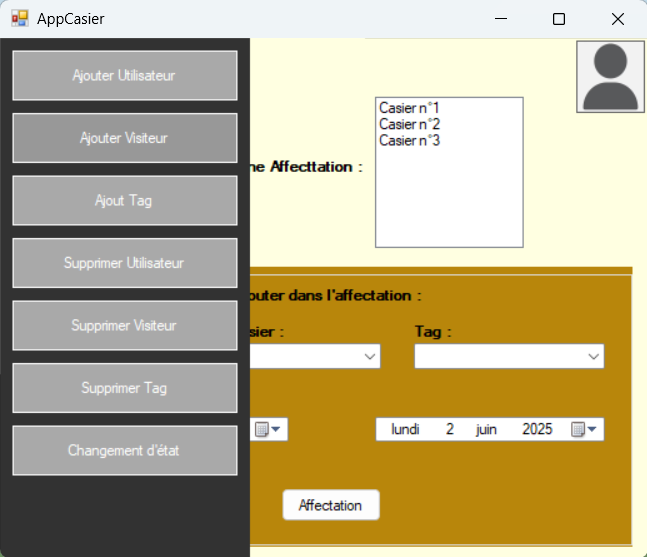
\includegraphics[width=0.7\textwidth]{../images/MenuIHM}
	\caption{Affichage du menu de l'application}
	\label{fig:PAM_APP_PP}
\end{figure}

\subsubsection{Classe pour le lecteur}

La classe Lecteur constitue un composant essentiel de l'application pour la gestion de la lecture des tags RFID via un port série. Elle encapsule toute la logique de communication avec un lecteur RFID physique connecté à un port COM. Lors de l’instanciation, elle configure le port série avec les paramètres fournis (nom du port et débit en bauds) et prépare la communication. 

Elle dispose de méthodes pour ouvrir et fermer le port série de manière sécurisée. Le mécanisme de lecture repose sur un événement déclenché automatiquement lorsque des données sont reçues. Une fois un tag détecté, les données sont filtrées et formatées pour extraire le numéro de tag, qui est stocké dans une variable dédiée. Un délai de 2 secondes est utilisé pour laisser au lecteur le temps de transmettre les données complètes avant leur traitement. 

La méthode lireTag() tente de lire un tag pendant une période maximale de 5 secondes, en vérifiant régulièrement si un tag a été capté. Si rien n'est détecté à temps, elle retourne false. La méthode IsConnected() quant à elle permet de tester la connexion au lecteur en essayant d’ouvrir et fermer le port série, ce qui est utile pour prévenir des erreurs de connexion matérielle. 

Dans la classe Lecteur, l'événement DataReceived du port série (SerialPort) est utilisé pour déclencher automatiquement une fonction lorsqu'une donnée arrive depuis le lecteur RFID. 

L’événement DataReceived est attaché dynamiquement dans la méthode lireTag() avec cette ligne : 

\begin{lstlisting}
m_SPort.DataReceived += eventDeLecture; 
\end{lstlisting}

Cela signifie que chaque fois que le lecteur envoie des données (par exemple, lorsqu'une carte RFID est scannée), la méthode eventDeLecture est automatiquement appelée en arrière-plan. 

La méthode eventDeLecture lit les données disponibles dans le tampon via m\_SPort.ReadExisting(), attend un court moment (2 secondes), puis traite ces données pour extraire le numéro du tag, en supprimant les caractères de début et de fin. 

Ce mécanisme basé sur les événements permet de ne pas bloquer l'interface utilisateur : l’application reste réactive pendant que le lecteur fonctionne. C’est un modèle asynchrone basé sur des interruptions matérielles, ce qui est courant pour les périphériques série. 

Une fois qu’un tag est lu ou que le délai expire, l’événement est détaché avec : 

\begin{lstlisting}
m_SPort.DataReceived -= eventDeLecture; 
\end{lstlisting}

Cela évite que le gestionnaire soit appelé plusieurs fois de manière indésirable, ce qui pourrait provoquer des lectures incorrectes ou redondantes. 

En résumé, l’appel de l’événement est dynamique, temporaire et utilisé pour capturer la donnée RFID dès qu’elle est disponible, sans bloquer l’exécution du reste du programme. 

Cette classe permet ainsi d’isoler et centraliser la logique liée à la lecture des identifiants RFID, facilitant leur intégration dans les différentes parties de l’application, tout en assurant un contrôle robuste sur les communications série. 

\subsubsection{Page Mainform}

Elle gère l'interface utilisateur après la connexion, permet l'affichage et la gestion des affectations de casiers à des visiteurs, et intègre un menu interactif (menu hamburger). 

Lors de l’exécution, le formulaire de connexion est d’abord affiché. Si l’utilisateur s’identifie correctement, la connexion à la base de données est ouverte et les éléments de l’interface (listes déroulantes, affectations) sont initialisés. 

La classe contient également la logique permettant : 

\begin{itemize}

\item Afficher les casiers disponibles ou affectés : La méthode afficherAffectation() est responsable d'afficher les casiers qui ont été affectés. Elle appelle la méthode db.listeAffectation() pour récupérer les numéros de casiers affectés depuis la base de données, puis les affiche dans un composant ListBox (nommé listBoxAffectation). Avant cela, elle vide le contenu du ListBox pour éviter les doublons à l'affichage. 

\item Gérer les affectations via des listes déroulantes (nom, casier, tag) : la méthode affichageSelection() permet d’alimenter trois listes déroulantes (ComboBox) avec des données disponibles : 
\begin{itemize}

\item cbAffectationNom pour les noms des visiteurs non affectés 

\item cbAffectationCasier pour les casiers libres 

\item cbAffectationTag pour les tags disponibles 

\end{itemize}

\item Ces listes sont remplies dynamiquement à partir de méthodes de la classe DatabaseConnection : recupNomPrenomVisiteurNonAffecté, recupNumCasierNonAffecté, recupNumTagNonAffecté. 

\item Vérifier la validité des dates sélectionnées : Dans la méthode btAffectation\_Click, plusieurs vérifications sont faites : 

\begin{itemize}

\item Les champs ne doivent pas être vides. 

\item La date de début doit être antérieure à la date de fin. 

\item La date de début doit être égale ou postérieure à la date actuelle. 

\end{itemize}

\item Ces contrôles permettent d’éviter des incohérences dans les enregistrements (comme des affectations expirées ou inversées). 

\item Alerter sur les affectations dépassées : la méthode affichageDatePasser() est appelée à l’ouverture de l’application. Elle interroge la base de données via db.affectationDateLimite() pour récupérer les casiers dont la date de fin est passée. Pour chaque casier, une fenêtre d’alerte (verifDate) est affichée, invitant l'utilisateur à réagir. Cela permet une gestion proactive des casiers non libérés à temps. 

\item De gérer la fermeture de session ou l’affichage du menu : Deux éléments importants permettent une interaction fluide avec l’application : 

\begin{itemize}

\item Le menu hamburger est initialisé via menu.InitializeHamburgerMenu(this) et peut être fermé avec FermetureMenu() ou FermetureMenuHamburger(). 

\item Un clic sur le logo (pbLogo\_Click) déclenche une boîte de dialogue de déconnexion (logout), permettant à l'utilisateur de se déconnecter de la session courante. 

\end{itemize}

\end{itemize}

La base de données est manipulée via une instance de la classe DatabaseConnection. La structure suit une logique événementielle typique de Windows Forms (gestionnaire de clics, timers, etc.). L’architecture montre un découpage clair entre logique métier et présentation, avec des appels aux classes secondaires pour les fonctionnalités spécifiques (connexion, menu, affichage des détails). La classe MainForm joue donc un rôle central dans l’application : elle coordonne l’interface utilisateur, la gestion des données (via la base), la sécurité (connexion/session), et le contrôle logique (vérifications, synchronisation des affichages, etc.). Elle s’assure que l’expérience utilisateur soit fluide, cohérente et conforme aux règles métier de l’application de gestion de casiers. 

\begin{figure}[H]
	\centering
	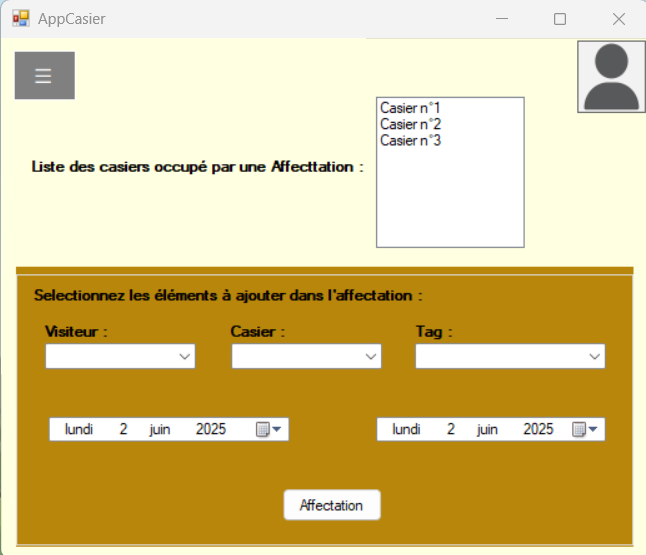
\includegraphics[width=0.7\textwidth]{../images/MainFormIHM}
	\caption{Page d'accueil de l'application}
	\label{fig:PA_APP_PP}
\end{figure}

\subsubsection{Page d'ajout de Visiteur}

Lorsque l'utilisateur ouvre la page "Ajout Visiteur", il doit saisir des informations comme le nom, le prénom, la compagnie, la plaque d’immatriculation et choisir un pays dans une liste déroulante. En fonction du pays sélectionné, l’application affiche un exemple de plaque correspondant au format utilisé dans ce pays, ainsi qu’un drapeau. 

Ce format est défini à l’aide d’une expression régulière (regex). Cette regex est chargée dynamiquement depuis une structure nommée PlaquesEuropeennes, qui contient pour chaque pays un format de plaque typique (par exemple, pour la France : deux lettres, trois chiffres, puis deux lettres, soit AB-123-CD). 

Quand l'utilisateur clique sur le bouton pour valider l'ajout du visiteur, le programme vérifie si le champ de la plaque est conforme à la regex du pays sélectionné. Si ce n’est pas le cas, il affiche un message d’erreur et bloque l’enregistrement. 

Par exemple, si l’utilisateur choisit l’Allemagne, la regex pourrait ressembler à \texttt{\^{}[A-Z]\{1,3\} [A-Z]\{1,2\} \textbackslash d\{1,4\}\$}, et il devra donc écrire une plaque comme B AB 1234. Toute autre forme entraînera un message comme "La plaque doit être sous la forme demandée !". 

Ce mécanisme permet de garantir que les plaques saisies sont réalistes et adaptées au pays, tout en améliorant l’expérience utilisateur avec un exemple visuel et un retour immédiat en cas d’erreur. 

\begin{figure}[H]
	\centering
	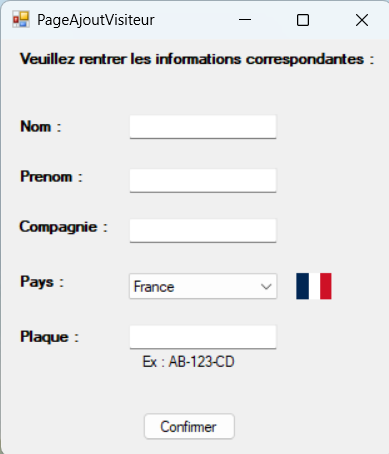
\includegraphics[width=0.6\textwidth]{../images/AjoutVisiteurIHM}
	\caption{Page d'ajout de visiteur}
	\label{fig:PAV_APP_PP}
\end{figure}


\subsubsection{Page d'ajout d'utilisateur}

La classe PageAjoutUtilisateur a pour objectif de permettre l’ajout d’un nouvel utilisateur dans la base de données de l’application. Elle centralise les interactions entre l’utilisateur et le système de gestion des utilisateurs via un formulaire simplifié.

Dès l’ouverture de la fenêtre, le constructeur de la classe initialise l’interface graphique et établit une connexion à la base de données via une instance de la classe DatabaseConnection. Cette étape est cruciale car elle prépare le système à effectuer des opérations de lecture et d’écriture dès que l'utilisateur interagit avec le formulaire.

L'intérêt de cette classe réside dans la méthode btAccepter\_Click, qui s’active lorsque l’utilisateur clique sur le bouton de validation. Cette méthode commence par une vérification des champs du formulaire (tbLogin, tbPassword, et cbRole). Si l’un de ces champs est vide, un message d’erreur est affiché, ce qui garantit que l’enregistrement ne sera pas incomplet.

Ensuite, une vérification est faite pour savoir si un utilisateur portant le même identifiant existe déjà dans la base. Cela permet d’éviter les doublons, assurant l’unicité du login utilisateur. Si un doublon est détecté, un message d’alerte est affiché.

Si toutes les vérifications sont passées avec succès, la méthode ajouterUtilisateur est appelée. Elle enregistre les informations du nouvel utilisateur (login, mot de passe, rôle) dans la base de données. En cas de réussite, une confirmation est affichée et la fenêtre se ferme automatiquement. En cas d’échec (par exemple si l’utilisateur a été ajouté entre-temps), un message d’erreur s’affiche.

\begin{figure}[H]
	\centering
	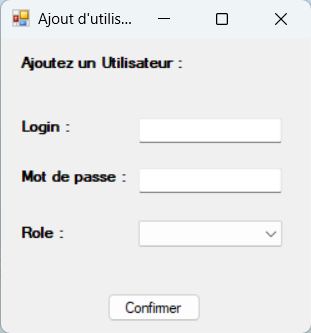
\includegraphics[width=0.6\textwidth]{../images/AjoutUserIHM}
	\caption{Page d'ajout d'utilisateur}
	\label{fig:PAU_APP_PP}
\end{figure}

\subsubsection{Page d'ajout tag}

La classe PageAjoutTag représente une fenêtre de formulaire dans une application Windows Forms destinée à l’ajout d’un tag RFID dans une base de données. Elle joue un rôle essentiel dans la gestion des identifiants utilisés par le système pour contrôler les accès ou associer des utilisateurs/visiteurs à des casiers. Cette classe illustre une bonne séparation des responsabilités entre l’interface utilisateur, la logique de lecture de tag, et la manipulation des données.

Lors de sa création, la classe reçoit deux objets en paramètres : une instance de MainForm et une de Lecteur. Cela permet à la fenêtre :

\begin{itemize}
\item de communiquer avec l’interface principale (actualisation des données après ajout)
\item d’interagir avec le lecteur de tags RFID pour lire automatiquement un tag
\end{itemize}

Elle configure également la fenêtre pour empêcher le redimensionnement, ce qui garantit une interface plus stable et maîtrisée.

Le bouton btAjoutTag déclenche la procédure d’ajout d’un tag. Plusieurs vérifications sont effectuées :

\begin{itemize}
\item Si le champ tbTag est vide, l’ajout est bloqué
\item Si le tag existe déjà (vérifié via db.verifTag()), l'utilisateur est informé
\item Si tout est correct, db.ajouterTag() est appelé pour insérer le tag dans la base, et la fenêtre se ferme ensuite
\end{itemize}

Cette logique permet de garantir l’intégrité des données, en évitant les doublons et les valeurs invalides.

Le bouton btSelectTag permet d’ouvrir une fenêtre lectureTag qui interagit avec un lecteur RFID pour récupérer un tag automatiquement. Cette fonctionnalité rend le processus plus fluide pour l’utilisateur, en évitant la saisie manuelle. Une fois le tag lu, il est affiché dans le champ de texte.

\begin{figure}[H]
	\centering
	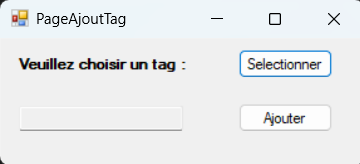
\includegraphics[width=0.6\textwidth]{../images/AjoutTagIHM}
	\caption{Page d'ajout de tag}
	\label{fig:PAT_APP_PP}
\end{figure}

\subsubsection{Page de suppressions (Utilisateur/Visiteur/Tag)}

Les trois classes pageSupprTag, pageSupprUtilisateur et pageSupprVisiteur partagent une structure très similaire car elles répondent au même objectif : permettre la suppression d’éléments (tags, utilisateurs, visiteurs) depuis l’interface de l’application.

Chacune hérite d’un formulaire Windows Forms et utilise une instance de la classe DatabaseConnection pour communiquer avec la base de données. Lors de l’ouverture du formulaire, une méthode spécifique remplit une liste déroulante (ComboBox) avec les éléments récupérés depuis la base. L’utilisateur sélectionne un élément, puis clique sur un bouton pour le supprimer. Si l’opération réussit, un message de confirmation s’affiche, sinon une erreur est signalée.

Ce fonctionnement uniforme permet de standardiser l’expérience utilisateur, de simplifier le développement et la maintenance, et de faciliter l’extension de l’application à d’autres entités à supprimer.

\begin{figure}[H]
	\centering
	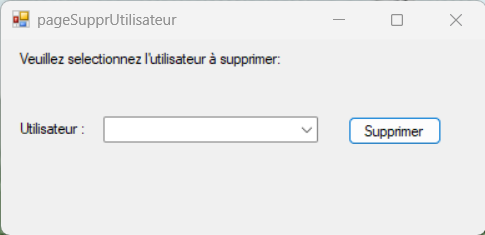
\includegraphics[width=0.7\textwidth]{../images/SupprUserIHM}
	\caption{Page de suppression d'utilisateurs}
	\label{fig:PSU_APP_PP}
\end{figure}

\begin{figure}[H]
	\centering
	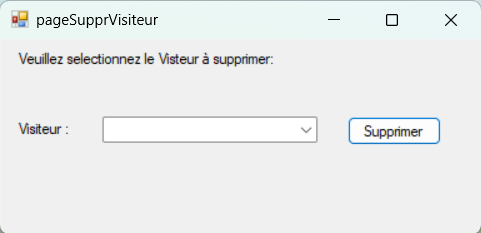
\includegraphics[width=0.7\textwidth]{../images/SupprVisiteurIHM}
	\caption{Page de suppression des visiteurs}
	\label{fig:PSV_APP_PP}
\end{figure}

\begin{figure}[H]
	\centering
	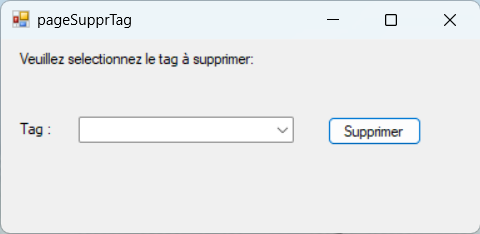
\includegraphics[width=0.7\textwidth]{../images/SupprTagIHM}
	\caption{Page de suppression des tags}
	\label{fig:PST_APP_PP}
\end{figure}

\newpage

\end{document}